%!TEX root = ../thesis.tex

\chapter{Anforderungsanalyse} % (fold)
\label{cha:anforderungsanalyse}

Um sich eine Vorstellung davon zu machen, wie ein System auszusehen hat und welche Komponenten dazu nötig sind um zwei oder mehrere sozialen Netzwerke zu verbinden, soll hierzu ein kleines Beispiel\footnote{Das vollständige Ablaufdiagramm befindet sich im Anhang \ref{sec:anforderungsanalyse_ablaufdiagramm}} konstruiert werden. 

\section{Neuen Beitrag verfassen} % (fold)
\label{sec:neuen_beitrag_verfassen}

% section neuen_beitrag_verfassen (end)

Alles beginnt damit, dass ein zum Beispiel ein Student im sozialen Netzwerk A im Forum zur Veranstaltung Telekooperation 1 eine Frage zur aktuellen Übung stellen will. Er geht zuerst in den passenden Thread und beginnt einen neuen Beitrag zu schreiben. Sobald er fertig ist, klickt er auf \enquote{Absenden} und sein Beitrag wird in der Datenbank des sozialen Netzwerkes A gespeichert und als neuer Eintrag im Thread angezeigt (siehe Abbildung \ref{fig:beutzer_erstellt_beitrag_a}).

\medskip

\begin{figure}[ht]
     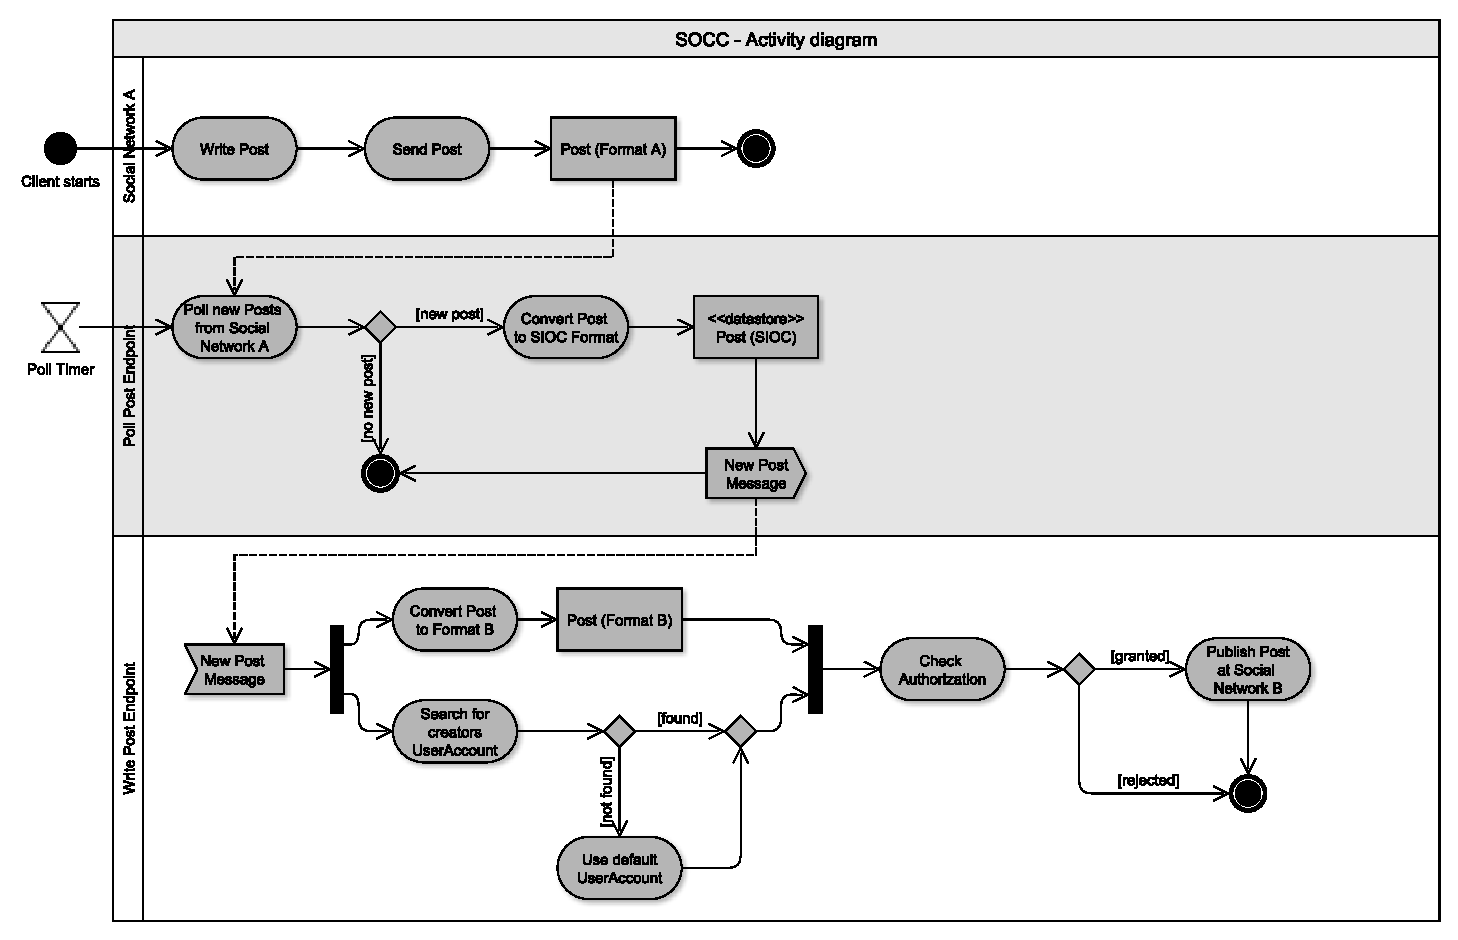
\includegraphics[
        width=\textwidth,
        keepaspectratio=true,
        clip=true,
        trim= 0 338 0 27
    ]{assets/images/activitydiagram_post_as_user_check_authorization.pdf}
    \caption{Benutzer erstellt einen Beitrag im sozialen Netzwerk A.}
    \label{fig:beutzer_erstellt_beitrag_a}
\end{figure}

\section{Beiträge von sozialen Netzwerk A lesen} % (fold)
\label{sec:beiträge_von_solzialen_netzwerk_a_lesen}


 Um diese Beitrag in das soziale Netzwerk B transferieren zu können, müssen zuerst die Daten über eine öffentliche Schnittstelle von den Servern des sozialen Netzwerks A heruntergeladen werden. Da in der Regel nicht automatisch bekannt ist, wann ein neuer Beitrag vorhanden ist, müssen die Server in zeitlichen Abständen abgefragt (polling genannt) und die zurückgelieferten Daten nach neuen Beiträgen durchsucht werden. Sind ein oder mehrere neue Beiträge gefunden worden, können diese nicht direkt an das soziale Netzwerk B geschickt werden, da sich diese in der Regel im verwendeten Datenformat unterscheiden. Diese müssen zuvor konvertiert werden.

\medskip

 Die einfachste Möglichkeit wäre nun die Daten von Format A nach Format B zu konvertieren. Bei zwei Formaten ist dies noch sehr einfach. Es müsste lediglich ein Konverter von Format A nach Format B und einer in die umgekehrte Richtung implementiert werden. Für den Fall, dass nun ein weiteres Netzwerk C unterstützt werden soll, würde ich die Anzahl an nötigen Konvertern auf Sechs erhöhen, wie Tabelle \ref{tbl:anzahl_konvertern_bei_drei_netzwerken} zeigt. 

 \medskip

\begin{table}[h]
    \centering
    \begin{tabular}{cc}
        A $ \Rightarrow $ B & A $ \Rightarrow $ C \\
        B $ \Rightarrow $ A & B $ \Rightarrow $ C \\
        C $ \Rightarrow $ A & C $ \Rightarrow $ B \\
    \end{tabular}
    \caption{Konverter bei Drei sozialen Netzwerken}
    \label{tbl:anzahl_konvertern_bei_drei_netzwerken}
\end{table}

 Nimmt man an $n_{sn}$ sei eine beliebige Anzahl Netzwerke, entspricht die Anzahl der notwendiger Konverter $ n_{k1}= n_{sn}*(n_{sn}-1) $, da für jedes Netzwerk ein Konverter in alle anderen Netzwerke erzeugt werden muss. Sollen nur Zwei oder Drei Netzwerke unterstützt werden ist der Aufwand noch sehr überschaubar, bei mehr kann dies aber sehr Aufwendig werden. 

\medskip

Eine elegantere Methode, welche die Anzahl zu implementierender Konverter in Grenzen halten kann, wäre die Einführung eines Zwischenformates. Geht man davon aus, dass die Daten aller Netzwerke nur in dieses Zwischenformat geschrieben und aus diesem gelesen werden müssen, würde sich der Aufwand auf maximal Zwei Konverter pro neuem Netzwerk reduzieren. Für eine beliebige Anzahl Netzwerke wären also $ n_{k2} = n_{sn} * 2 $ Konverter nötig. Nachteile hätte dieser Ansatz nur für $ n_{sn}=2 $ und $ n_{sn}=3$ , da in diesen Fällen mehr beziehungsweise gleich viele Konverter gegenüber der ersten Methode erforderlich wären. Erhöht man die Anzahl Netzwerke jedoch nur geringfügig, sinkt die Menge an Konvertern sichtbar. Für $ n_{sn} = 4 $ wären es $ n_{k2} = 8 $ statt $ n_{k1} = 12 $ und für $ n_{sn} = 5 $ ergibt sich $ n_{k2} = 10 $ statt $ n_{k1} = 20 $ Konvertern. Gleichzeitig können so syntaktische Unterschiede in den einzelnen Formaten angeglichen werden, was sie leichter handhabbar macht.

\medskip

\begin{figure}[h]
     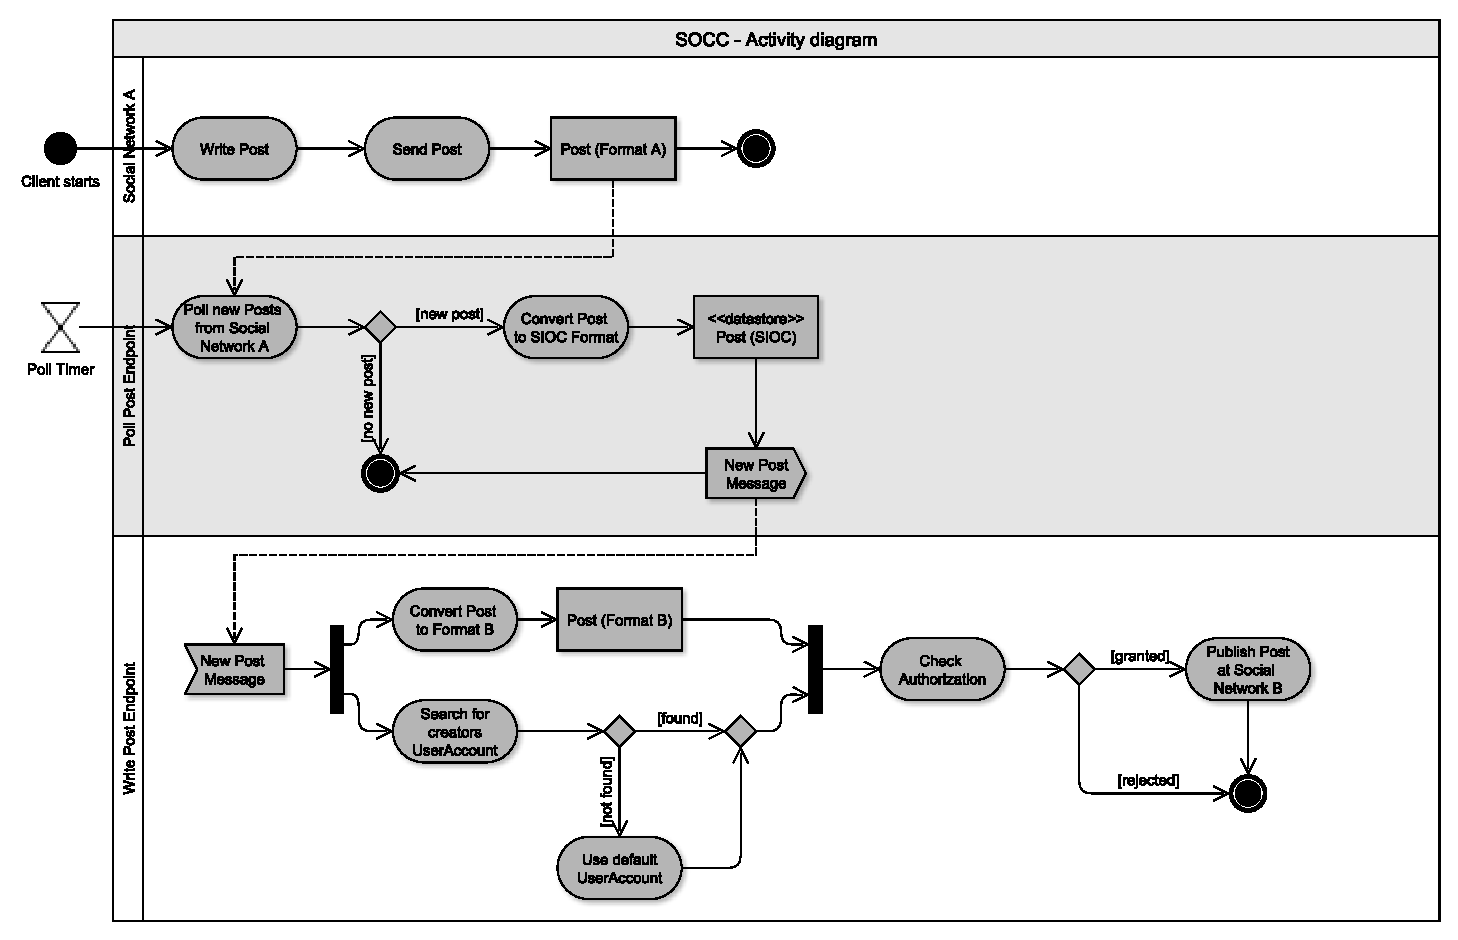
\includegraphics[
        width=\textwidth,
        keepaspectratio=true,
        clip=true,
        trim= 0 193 0 113
    ]{assets/images/activitydiagram_post_as_user_check_authorization.pdf}
    \caption{
        Lesen des erstellten Beitrags und konvertieren in das Zwischenformat.
    }
    \label{fig:lesen_von_beitrag_und_convertieren}
\end{figure}


Liegen nun alle Daten in diesem Zwischenformat können diese an einen zentralen Ort gespeichert werden. So ist es denkbar diese Daten zum Beispiel für die Suche nach ähnlichen oder inhaltlich zusammenhängenden Beiträgen weiter zu verwenden. Die Möglichkeiten sind hier vielfältig.

\medskip

Da mit diesem Projekt auch eine automatische Synchronisation neuer Beträge zwischen unterschiedlichen sozialen Netzwerken ermöglicht werden soll, muss das Eintreffen eines neuen Betrags an die entsprechenden Stellen weitergereicht werden. Da dieser Zeitpunkt nicht im Vorneherein bekannt ist würde sich hier ein Event-basierter Ansatz anbieten. So entsteht eine zeitliche Entkopplung des Lesens und Schreibens von Beträgen. Der Einsatz eines \enquote{Publish-Subscribe}-Mechanismus wäre hier ebenfalls von großen Vorteil, da so die Beträge eines sozialen Netzwerkes mit mehreren Synchronisiert werden kann. Der komplette Ablauf des Lesens, Konvertierens und bekanntmachen neuer Beiträge wird in Abbildung \ref{fig:lesen_von_beitrag_und_convertieren} noch einmal graphisch dargestellt.

% section beiträge_von_solzialen_netzwerk_a_lesen (end)

\section{Beitrag an soziales Netzwerk B weiterleiten} % (fold)
\label{sec:beitrag_an_soziales_netzwerk_b_weiterleiten}


Wurde nun ein Event, dass ein neuer Beitrag gelesen wurde, abgeschickt wird dieser über den besagten \enquote{Publish-Subscribe}-Mechanismus an alle dadurch verbundenen Endstellen weitergeleitet. Dieses konvertieren nun den Beitrag in das entsprechende Format des soziale Netzwerks und holen sich alle nötigen Information um diesen dort hin zuschicken. Eine wünschenswerte Erweiterung hierbei wäre \todo{Quelle suchen}, wenn der so geschriebene Beitrag dann so erscheinen würde, als hätte der Autor des ursprünglichen Beitrags ihn selber geschrieben. Hierzu müssten die einzelnen Benutzer das System, zum Beispiel durch das hinterlegen von Access Token\footnote{\url{http://oauth.net/}} oder anderen Authentifizierungsparameter, autorisieren in ihren Namen Nachrichten zu schreiben. Diese könnten dann anhand der Benutzerkennung herausgesucht und benutzt werden. 

\begin{figure}[h]
     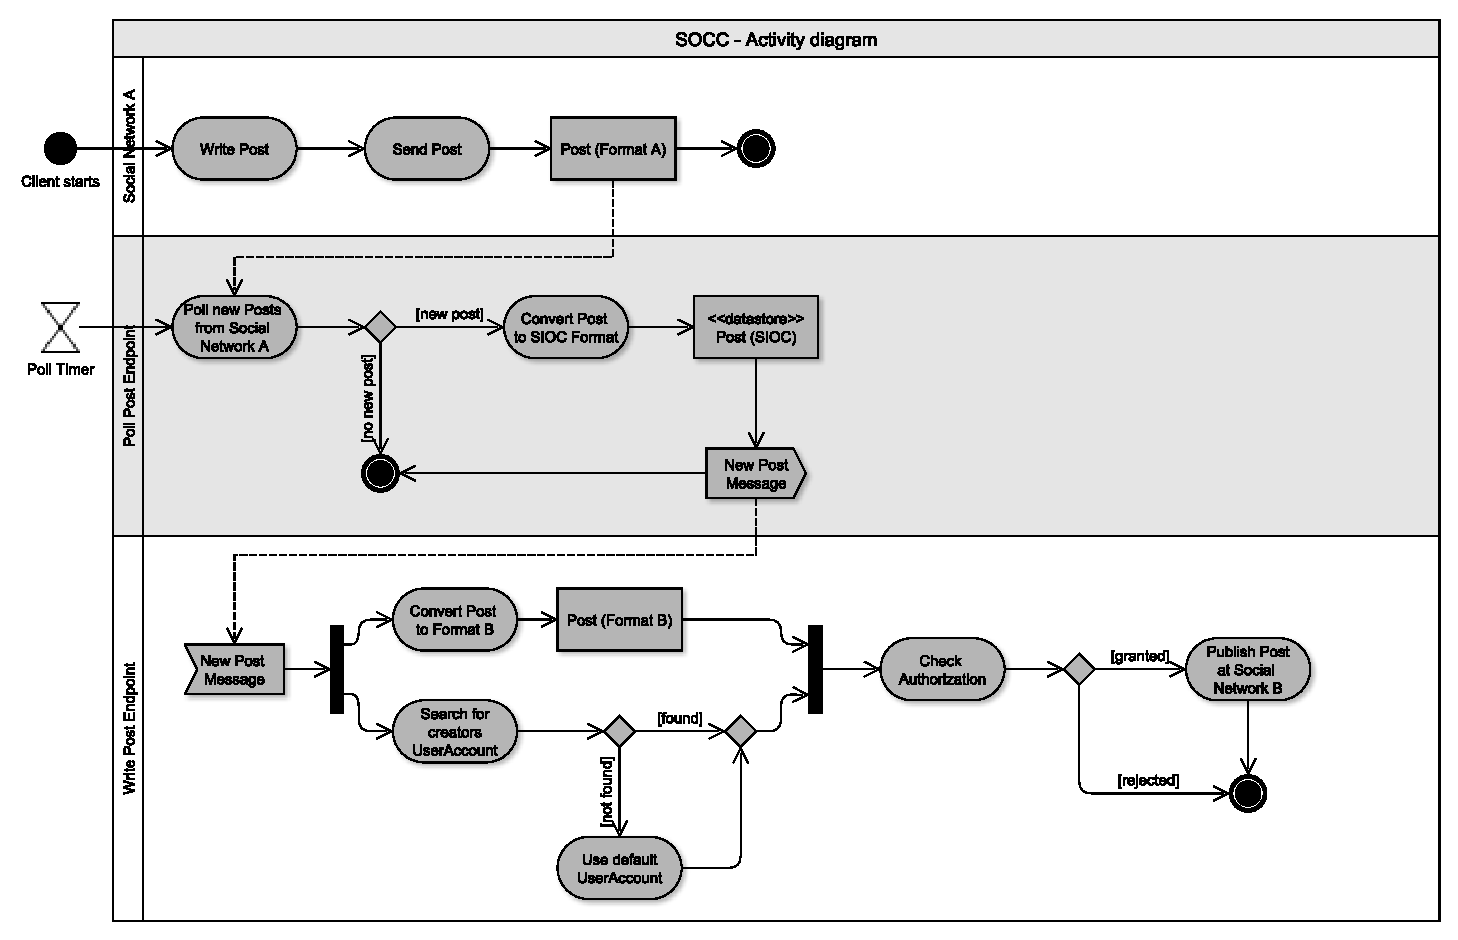
\includegraphics[
        width=\textwidth,
        keepaspectratio=true,
        clip=true,
        trim= 0 0 0 257
    ]{assets/images/activitydiagram_post_as_user_check_authorization.pdf}
    \caption{
        Konvertierten des Beitrags in das Format B und schreiben in das soziale Netzwerk B
    }
    \label{fig:konvertieren_formatb_und_schreiben}
\end{figure}

% section beitrag_an_soziales_netzwerk_b_weiterleiten (end)

% chapter anforderungsanalyse (end)
